\chapter{可靠性}
\label{chap:trust-reliability}

邮件分类器报告“垃圾邮件概率为0.9”，使用者可能据此自动隔离邮件。但0.9究竟代表什么：在相似情形中大约九成是垃圾邮件，还是模型内部的一个较大分数？如果换成一段生成式回答，某个词的概率很高，又能否说明整段内容正确？要依赖不确定性输出，需要先明确它描述的事件，再检验它与实际结果的关系。

本章讨论的\term{可靠性}（reliability），是指模型在约定的使用条件下，预测及据此作出的决策能否满足明确的质量与风险要求。要求可以落在概率的频率含义、预测范围的覆盖程度，或自动处理的损失上。判断可靠性需要同时说明这些要求和成立的条件，不能只给模型一个笼统的“可信”评分。

在第~\ref{chap:trust-foundations}章的三层架构中，可靠性主要属于系统属性或规范要求层：系统需要明确概率、预测范围或自动决策应达到什么标准。校准、覆盖和决策风险的检验与保证位于证据能力层，用来判断这些标准得到多强的支持。抽样关系、模型版本、阈值或反馈条件一旦改变，原结论可能失效，因而还要在失效、处置与生命周期层规定复验与限制使用的触发条件。

不确定性输出为这一判断提供线索：模型是否知道自己可能出错，所给范围是否反映尚未确定的结果。但线索本身也可能失真。第~\ref{sec:reliability-uncertainty}节说明不确定性的来源与估计；第~\ref{sec:reliability-evaluation}节从输出的数值含义、决策用途和适用范围检验这些估计；第~\ref{sec:reliability-guarantee}节再讨论如何在明确假设下构造满足覆盖或决策风险要求的程序。估计回答模型表达了什么，检验回答这种表达是否得到数据支持，保证则回答什么条件能够支持进一步的使用承诺。

图~\ref{fig:trust-reliability-review}把可靠性问题放回邮件处理场景：证据足够时按规则自动隔离，证据不足时转交复核。图标只是当前教学情景中的不同线索，不能把“带有宣传内容”直接当成垃圾邮件的判据。分流是否有价值，要在第~\ref{sec:reliability-selection-evaluation}节同时检查自动处理的比例与接受部分的风险。

\begin{figure}[!htb]
  \centering
  \bookdraftgraphic{figures/02-foundations/03-trustworthiness/generated/v1r3-reliability-story.png}
  \caption{按判断依据分配自动处理与复核。单个标记表示当前规则接受的判断，两个不同形状的标记表示仍待辨别的候选；上方邮件进入可恢复的隔离文件夹，下方交给人工。此图引入邮件处理情景，分流本身不证明可靠，也不假定人工无误；处理比例与选择性风险的计数见图~\ref{fig:trust-selective-risk-coverage}。}
  \label{fig:trust-reliability-review}
\end{figure}

\section{不确定性的来源与估计}
\label{sec:reliability-uncertainty}

可靠性需要相对于具体要求判断：概率是否有可信的频率含义、预测范围是否覆盖实际结果、采用预测作出的决策是否满足风险限制。不确定性描述模型对结果尚有多大把握，是建立这些判断的起点，却不等于可靠性本身。

模型不能确定结果，可能是当前信息不足以唯一决定结果，也可能是有限训练数据尚未让模型学会已有规律。这两种来源需要分别刻画：前者考察给定输入时结果仍有多大波动，后者考察仍有哪些不同模型与已知数据相容。本节先建立这一区分，再讨论两类来源的估计方法；这些估计是否兑现其含义，留到下一节用独立数据检验。

\subsection{不确定性的来源}
\label{sec:reliability-uncertainty-sources}

设输入为$\bm{x}$，目标为$y$，已有训练数据为$\mathcal D$。即使输入完全相同，结果也可能不同。例如，现有邮件特征没有包含发送者的真实意图，相同文本可能出现在正常通知和诈骗邮件中。相对于当前观测，仍然存在的结果随机性称为\term{偶然不确定性}（aleatoric uncertainty）。它不一定在增加观测信息后仍不可减少。

另一种不确定性来自知识不足：有限数据可能支持多个不同预测模型。补充相关样本后，模型之间的分歧可能减小，这通常称为\term{认知不确定性}（epistemic uncertainty）。两者是相对于观测和模型假设的区分，不能仅由一次预测分数唯一识别。

对邮件分类器，可以固定可见特征来理解这一区别。一种情况是同样的文字既可能出现在正常通知中，也可能被用于诈骗；即使充分掌握这类文字的统计规律，仅凭这些特征仍无法唯一判断。另一种情况是某种新语言的训练邮件很少，多个模型对相同内容给出不同判断；增加有标签的相关邮件，可能减少这部分知识不足。前者需要表达给定信息下的结果分布，后者需要表达对预测规律的把握程度。

区分来源并不意味着能直接测出各自大小。真实条件分布通常未知，模型还可能遗漏重要因素，因此实践中得到的是依赖模型假设的估计。参数后验、模型集成和条件分布学习都是建立这种估计的手段；它们本身不构成新的不确定性类别。近似计算也会产生误差，但这种估计误差应与被估计的不确定性分开。

图~\ref{fig:trust-uncertainty-sources}固定邮件任务比较两种信息缺口：左侧缺少区分真实意图的特征，右侧缺少能够约束候选模型的相关数据。增加同一类训练记录可能减少后者，却不自动补上前者缺少的观测信息。

\begin{figure*}[htbp]
  \centering
  % 真矢量机制对照；固定模型与候选模型的内部网格仅为对象图标。
% 右侧比例精确为.2/.5/.8；它们是教学构造，不是后验抽样。
\begin{tikzpicture}[figure picture,foundation picture,
 font=\figurefont\mdseries\fontsize{9}{11}\selectfont,
 trust module/.style={draw=FigureStroke,line width=1pt,rounded corners=1.5mm,fill=white},
 trust wire/.style={draw=FigureStroke,line width=.65pt},
 trust mesh node/.style={circle,draw=FigureStroke,line width=.65pt,fill=white,minimum size=1.8mm,inner sep=0pt}]
 \path[use as bounding box] (0,-2) rectangle (169,59);
 \node at (40,55) {偶然不确定性};
 \node at (127,55) {认知不确定性};
 \draw[draw=FigureMuted,line width=.6pt] (82,-1)--(82,58);
 \draw[trust module,fill=white] (1,20) rectangle (15,34);
 \node at (8,27) {$\bm x$};
 \draw[trust module] (25,12) rectangle (51,42);
 \node at (38,37.5) {固定模型$f$};
 \node at (38,31.5) {$p(y\mid\bm x)$};
 \foreach \xx/\yy/\id in {30/19/a,30/24/b,38/16/c,38/21.5/d,38/27/e,46/19/f,46/24/g}{
  \coordinate (fixed-\id) at (\xx,\yy);
 }
 \foreach \i in {a,b}{\foreach \j in {c,d,e}{\draw[trust wire] (fixed-\i)--(fixed-\j);}}
 \foreach \i in {c,d,e}{\foreach \j in {f,g}{\draw[trust wire] (fixed-\i)--(fixed-\j);}}
 \foreach \id/\col in {a/FigureBlue,b/FigureBlue,c/FigureRed,d/FigureRed,e/FigureRed,f/FigureYellow,g/FigureYellow}{\node[trust mesh node,fill=\col] at (fixed-\id) {};}
 \draw[trust module,fill=FigureBlueFill] (61,34) rectangle (78,46);
 \draw[trust module,fill=FigureRedFill] (61,8) rectangle (78,20);
 \node at (69.5,40) {$y=0$};
 \node at (69.5,14) {$y=1$};
 \draw[foundation flow] (15,27)--(25,27);
 \draw[foundation flow] (51,31) to[out=0,in=180] (61,40);
 \draw[foundation flow] (51,23) to[out=0,in=180] (61,14);
 % 相关数据D分叉至三个候选模型，不画候选之间的连接。
 \draw[trust module,fill=white] (87,18) rectangle (101,36);
 \foreach \dx/\dy in {0/2,1.8/1,3.6/0}{
  \draw[trust wire,fill=white,rounded corners=.4mm] ({89+\dx},{25+\dy}) rectangle ({94+\dx},{32+\dy});
 }
 \draw[trust wire] (93.5,30)--(96.5,30) (93.5,28.6)--(96.5,28.6) (93.5,27.2)--(96,27.2);
 \node at (94,21.5) {$D$};
 \foreach \yy/\m/\prob/\len in {44/1/0.2/4.4,27/2/0.5/11,10/3/0.8/17.6}{
  \draw[trust module] (112,{\yy-7}) rectangle (131,{\yy+7});
  \node[anchor=north west,inner sep=0pt] at (113.5,{\yy+6}) {$f_{\m}$};
  \foreach \xx/\dy/\id in {115.5/-2/a,121.5/1/b,121.5/-2/c,121.5/-5/d,127.5/-2/e}{
   \coordinate (candidate-\m-\id) at (\xx,{\yy+\dy});
  }
  \foreach \i in {b,c,d}{\draw[trust wire] (candidate-\m-a)--(candidate-\m-\i)--(candidate-\m-e);}
  \foreach \id/\col in {a/FigureBlue,b/FigureRed,c/FigureRed,d/FigureRed,e/FigureYellow}{\node[trust mesh node,fill=\col] at (candidate-\m-\id) {};}
  \fill[FigureRedFill] (144,{\yy-1.5}) rectangle ({144+\len},{\yy+3.5});
  \draw[draw=FigureStroke,line width=.9pt,rounded corners=.5mm] (144,{\yy-1.5}) rectangle (166,{\yy+3.5});
  \draw[draw=FigureRed,line width=.8pt] ({144+\len},{\yy-1.5})--({144+\len},{\yy+3.5});
  \node at (155,{\yy-5.5}) {$p_{\m}=\prob$};
  \draw[foundation flow] (131,\yy)--(144,\yy);
 }
 \draw[foundation flow] (101,31) to[out=0,in=180] (112,44);
 \draw[foundation flow] (101,27)--(112,27);
 \draw[foundation flow] (101,23) to[out=0,in=180] (112,10);
\end{tikzpicture}%

  \caption{偶然不确定性与认知不确定性的区别。左侧同一可见特征可能对应正常通知或诈骗意图，固定模型也需表达结果分布；右侧相关样本不足，三个候选模型给出不同预测，$p_m$简写$p_m(y=1\mid\bm x)$。概率0.2、0.5、0.8为教学构造，条长示意预测分歧，不是实测值或后验抽样。两种来源均相对于当前观测与模型假设而言。}
  \label{fig:trust-uncertainty-sources}
\end{figure*}

\subsection{认知不确定性的估计}
\label{sec:reliability-epistemic-estimation}

对于知识不足，仅保留一个拟合结果会隐藏其他可能的解释。估计认知不确定性的一个思路，是保留多个与数据相容的模型，观察它们对同一输入是否给出相同预测。参数可以相差很大而预测相同，因此与决策有关的是预测分歧，不能只看参数数值的离散程度。

在贝叶斯建模中，设$\bm{\theta}$为模型参数，$p(\bm{\theta}\mid\mathcal D)$为参数后验，预测分布通过积分得到
\begin{equation}
 p(y\mid\bm{x},\mathcal D)
 =\int p(y\mid\bm{x},\bm{\theta})
       p(\bm{\theta}\mid\mathcal D)\,\mathrm d\bm{\theta}.
 \label{eq:reliability-posterior-predictive}
\end{equation}
每个候选参数给出一个条件预测，后验权重表达数据对候选参数的支持。对于二阶矩存在的实值目标，全方差公式进一步给出
\begin{equation}
 \begin{aligned}
 \operatorname{Var}(y\mid\bm{x},\mathcal D)
 ={}&\mathbb E_{\bm{\theta}\mid\mathcal D}
       \operatorname{Var}(y\mid\bm{x},\bm{\theta})\\
 &+\operatorname{Var}_{\bm{\theta}\mid\mathcal D}
       \mathbb E(y\mid\bm{x},\bm{\theta}).
 \end{aligned}
 \label{eq:reliability-variance-decomposition}
\end{equation}
第一项平均各模型内部的结果波动，对应所建模型中的偶然不确定性；第二项刻画各模型预测均值的分歧，对应参数知识不足带来的预测方差。这里把总预测方差拆成两个来源，而不是把总方差都称为认知不确定性。这个分解在给定概率模型中成立，却不证明模型已经包含现实中全部不确定性。若所有候选模型都遗漏同一个因素，第二项很小也可能伴随系统性错误。

式~\eqref{eq:reliability-posterior-predictive}说明了理想的计算对象，却没有解决计算困难。深度网络的参数很多，后验通常无法直接积分。若只保留使后验密度最大的一个参数，预测就忽略了其他仍与数据相容的解释。实际方法需要在计算预算内，保留一部分参数不确定性。

一种做法是用容易抽样的分布$q_{\bm{\phi}}(\bm{\theta})$逼近后验，其中$\bm{\phi}$控制近似分布。最小化$q_{\bm{\phi}}$到后验的KL散度，等价于最小化
\begin{equation}
 \mathcal J(\bm{\phi})
 =-\mathbb E_{q_{\bm{\phi}}}\log p(\mathcal D\mid\bm{\theta})
   +\operatorname{KL}\bigl(q_{\bm{\phi}}(\bm{\theta})
                    \,\|\,p(\bm{\theta})\bigr).
 \label{eq:reliability-variational-objective}
\end{equation}
第一项要求抽出的模型解释数据，第二项限制近似分布偏离先验的程度；被省略的
$\log p(\mathcal D)$与$\bm{\phi}$无关。这种近似把难积分的问题转成优化问题，但近似族可能过于狭窄。例如，彼此独立的单峰参数分布未必能表达多种相距很远的解释。优化收敛也不能消除近似族本身的限制。

Gal和Ghahramani从这一思路解释了特定设置下的dropout训练，并提出在预测时保留随机失活、进行多次前向计算来估计不确定性。这一方法通常称为\term{蒙特卡洛失活}（Monte Carlo dropout, MC dropout）：同一输入经过不同随机掩码，产生多个预测，再用这些预测近似积分。它复用了常见训练机制，但贝叶斯解释依赖相应的近似模型与正则化设置，不能把任意已有网络随意打开dropout所得的波动都当成正确后验\scite{gal2016dropout}。

若进行$M$次前向计算，第$m$次得到类别分布$p_m(y\mid\bm{x})$，其平均$\bar p(y\mid\bm{x})=M^{-1}\sum_{m=1}^{M}p_m(y\mid\bm{x})$近似预测分布。增加$M$可以减小给定近似分布下的蒙特卡洛误差，却不能修正先验、似然或近似族的错误。对延迟敏感的系统，还需要将重复前向计算的成本与拒答带来的收益一同评价。

另一条路径不要求显式近似参数后验，而是保留多个独立优化得到的模型。\term{深度集成}（deep ensembles）对多个网络的预测分布求平均，用模型之间的分歧补充单个网络的输出。Lakshminarayanan等将独立初始化、概率评分训练与集成预测结合，为深度网络提供了易于实现和并行训练的不确定性基线\scite{lakshminarayanan2017ensembles}。

对于第$m$个回归模型，设输出均值$\mu_m(\bm{x})$和方差$v_m(\bm{x})$。等权混合的均值与方差为
\begin{equation}
 \begin{aligned}
 \bar\mu(\bm{x})&=\frac1M\sum_{m=1}^{M}\mu_m(\bm{x}),\\
 \bar v(\bm{x})&=\frac1M\sum_{m=1}^{M}v_m(\bm{x})
  +\frac1M\sum_{m=1}^{M}
       \bigl(\mu_m(\bm{x})-\bar\mu(\bm{x})\bigr)^2.
 \end{aligned}
 \label{eq:reliability-ensemble-variance}
\end{equation}
这正是混合分布的全方差分解。作为教学例子，两个模型的预测均值为0和2，方差均为1，混合均值便是1，方差为$1+1=2$。只平均方差会漏掉均值分歧；只计算均值分歧又会漏掉各模型内部的结果波动。

集成成员独立初始化，不意味着它们的错误在现实数据上相互独立。相同训练集、架构和损失可能诱发共同的盲点。多个模型一致地给出错误答案时，集成分歧仍然很小。因此，MC dropout与深度集成主要提供可计算的概率表达和分歧信号，其价值要由校准、拒答效果及分布变化下的检验确认。

\subsection{偶然不确定性的刻画}
\label{sec:reliability-aleatoric-estimation}

上一小节改变候选模型，观察预测是否一致；这里固定一个候选模型，考察它认为同一输入下结果还可能怎样变化。这对应式~\eqref{eq:reliability-variance-decomposition}中的模型内部波动。分类任务可以输出类别概率，回归任务则需要给出条件分布或预测范围。对于输入相关的噪声，可以同时学习条件均值和条件方差；若只关心结果落在哪个范围内，也可以直接拟合分位点，而不指定完整分布。

若假定$y\mid\bm{x}$服从均值$\mu(\bm{x})$、方差$v(\bm{x})>0$的正态分布，忽略常数后的单样本负对数似然为
\[
 \frac{(y-\mu(\bm{x}))^2}{2v(\bm{x})}
       +\frac12\log v(\bm{x}).
\]
增大方差可以降低大残差的第一项，却会增大第二项；两个部分共同约束模型，避免通过无限放大方差解释一切误差。不过，单个正态分布难以表达多峰结果。如果一封邮件可能属于两种完全不同的处理路径，用一个中间均值和很大的方差概括，未必适合后续决策。

不愿完整指定分布形状时，可以直接学习所需分位点。对$\tau\in(0,1)$，\term{分位数损失}（pinball loss）写为
\[
\rho_\tau(u)=u\bigl(\tau-\mathbb I\{u<0\}\bigr),
 \qquad u=y-q_\tau(\bm{x}).
\]
在损失期望存在时，按真实分布最小化该期望，会得到一个$\tau$分位点：目标值不大于该位置的概率至少为$\tau$，不小于该位置的概率至少为$1-\tau$。高分位点对低估惩罚更重，低分位点对高估惩罚更重。训练上下两个分位点即可形成随输入变化的区间，但有限数据、模型限制和优化误差都可能使实际覆盖偏离目标，后面需要独立校准补上这一环。

这些方法估计的是给定输入时的结果波动，但学习到的方差和分位点本身也会受知识不足影响，不能把一个网络输出的方差直接视为真实偶然不确定性。若把多个候选模型的结果分布混合，最终预测范围就同时反映模型内部波动和模型间分歧，仍需在未用于拟合的数据上检查。预测区间覆盖的是未来目标；参数置信区间或可信区间描述的是参数信息。将参数区间代入一个预测值，并不一定覆盖额外的结果噪声。

对生成模型，概率对象尤其重要。设回答为词元序列$(w_1,\ldots,w_T)$，其概率是条件词元概率的乘积。这个概率衡量模型偏好生成该序列的程度，不能直接当作陈述真实的概率。语义相同的答案还可能有许多表达方式。评价时应确定对象是一个事实主张、一个完整答案，还是完成任务的最终结果，再选择相应评分。

生成任务中的可靠性检验必须把完整程序冻结为评价对象，包括模型版本、提示、检索来源、
采样规则、重试次数、答案筛选和事实核验器。若事件定义为“回答中的每项事实主张均被
指定来源支持”，就应先规定怎样切分主张、哪些来源合格以及评判者如何处理分歧，再在
未参与这些选择的数据上估计该事件的风险。评判者本身的漏报与误报属于测量误差，不能
隐藏在一个笼统的正确率中。

同一程序还可以输出语义不确定性或拒答分数，并按第~\ref{sec:reliability-selection-evaluation}节
的方式检验：固定阈值后，报告自动回答部分的事实错误风险、处理比例和转人工成本。
这给出了章首生成问题的正面接口，但不把低词元熵、低语义分歧或高评判分数直接解释为
事实正确；每一种分数都必须通过其声称控制的事件来验证。

\section{可靠性的检验}
\label{sec:reliability-evaluation}

得到概率、区间或分歧分数之后，需要用已知结果检验它们。检验先从输出的数值含义入手，例如报告0.9的事件是否约有九成发生。

数值含义得到支持，仍不能说明分数适合决策。还要检查它能否找出较高风险的预测，使拒答确实降低自动处理风险。

上述证据如果只在总体上成立，仍可能掩盖重要群体或使用条件中的失败，因此还要在这些局部条件下复测。前两个角度分别评价输出本身和输出的决策用途，这一角度则检查前两类证据的适用范围，并不是另造一个综合分数。

三类检验都需要职责明确的数据。模型拟合、概率修正和阈值选择应在最终测试之前完成，不能在测试结果中反复选择有利设置后，仍将它们当作独立评价。生成任务还应固定正确性定义、评判者和采样规则。事实是否有来源、是否被来源支持、是否在现实中正确，是不同判断，不能只用字符串匹配覆盖全部要求。本节的“检验”包括指标估计与诊断；涉及达标与否的统计结论时，还需要给出抽样条件与估计误差。

\subsection{概率与预测范围的检验}
\label{sec:reliability-output-evaluation}

不确定性小意味着模型给出的范围集中，并不意味着范围的位置正确。反过来，一个覆盖所有可能标签的集合可以永远覆盖真实标签，却无法帮助选择行动。因此，可靠性既需要符合承诺，也需要保留足够的信息量。

概率校准的正式定义与适当评分背景见
\BookDefinitionRef{def:statistics-probability-calibration}{第一卷“随机变量”章的“概率校准”定义}。
对二分类，令$y\in\{0,1\}$，$p(\bm{x})$为预测事件$y=1$的概率。当前定义特化为
\begin{equation}
 \mathbb E[y\mid p(\bm{x})]=p(\bm{x})
\quad\text{相对于当前联合分布几乎必然成立},
 \label{eq:reliability-calibration}
\end{equation}
这就是本章所说的\term{校准}（calibration）：具有相同预测概率的样本，在总体中有对应的事件频率。连续分数下，条件期望的表述避免了把零概率事件直接当作普通频率计算。

一个始终输出总体正例比例的预测器也可能校准，却不能区分不同输入。校准与区分能力需要分别检查；同样，平均覆盖、个体信息量和决策损失也承担不同职责。Guo等对现代神经网络校准的研究说明，较好的分类表现并不自动带来恰当的概率表达\scite{guo2017calibration}。

图~\ref{fig:trust-calibration-discrimination}展示了这种区别。即使概率与总体频率相符，也仍要检查分数能否区分具有不同风险的输入。

\begin{figure*}[t]
  \centering
  % 左图为构造函数，右图为两个等大群体的总体概率；不含观测数据。
\begin{tikzpicture}[figure picture,foundation picture]
 \path[use as bounding box] (0,-8) rectangle (168,53);
 \draw[foundation axis] (10,0)--(72,0) node[right] {$p$};
 \draw[foundation axis] (10,0)--(10,46);
 \node[anchor=south west] at (5,48) {事件频率};
 \draw[FigureBlue,line width=1.1pt] (10,0)--(68,42);
 \draw[FigureRed,line width=1.1pt,dashed]
  plot[domain=0:1,samples=41] ({10+58*\x},{42*\x*\x});
 \node[anchor=west] at (16,37) {理想校准};
 \node[anchor=west] at (44,9) {过度自信};
 \node[below] at (10,0) {$0$}; \node[below] at (68,0) {$1$};
 \node[left] at (10,42) {$1$};
 \draw[draw=FigureGrid,line width=.6pt] (85,-5)--(85,49);
 \node at (116,43) {$\pi_1=0.2$};
 \node at (150,43) {$\pi_2=0.8$};
 \node[anchor=east] at (100,26) {常数};
 \node[foundation node,fill=FigureBlueFill,minimum width=26mm] at (116,26) {$p=0.5$};
 \node[foundation node,fill=FigureBlueFill,minimum width=26mm] at (150,26) {$p=0.5$};
 \node[anchor=east] at (100,8) {分组};
 \node[foundation node,fill=FigureRedFill,minimum width=26mm] at (116,8) {$p=0.2$};
 \node[foundation node,fill=FigureRedFill,minimum width=26mm] at (150,8) {$p=0.8$};
\end{tikzpicture}

  \caption{校准与区分能力的区别。左侧实线是理想校准关系，虚线是构造的过度自信曲线，二者不来自实验。右侧假设两个等大群体的正例比例分别为20\%和80\%；始终输出0.5的预测器在总体上校准，按组输出0.2与0.8的预测器同样校准，却能区分两组的风险。}
  \label{fig:trust-calibration-discrimination}
\end{figure*}
\FloatBarrier

\paragraph{概率校准的经验修正}

若分类排序较好而概率偏大，可以在独立校准数据上拟合后处理参数。例如，温度缩放用正数$t$调整未归一化类别对数分数$z_k(\bm{x})$（logit）：
\[
 p_t(y=k\mid\bm{x})
 =\frac{\exp(z_k(\bm{x})/t)}
        {\sum_j\exp(z_j(\bm{x})/t)}.
\]
在校准数据上最小化负对数损失可以选择$t$。正温度不改变同一输入中类别分数的大小顺序，因此保留最大概率类别，却改变概率的集中程度。若系统按固定概率阈值隔离邮件或拒答，实际行动仍可能改变，需要重新检验第~\ref{sec:trust-context}节中的行动损失。该过程改善的是数据支持下的概率表达，本身不提供任意新分布下的校准保证。

当$t>1$时，分数差被缩小，分布变得平缓；当$0<t<1$时，分布更集中。一个参数使方法不易在小校准集上过拟合，但也限制了能修复的错误：某些类别过度自信、另一些类别不足自信时，单一温度未必足够。更灵活的类别相关变换或单调映射能够修正更复杂偏差，却增加估计难度，甚至改变原有决策边界。选择复杂度应由独立评价支持，不能仅看校准集损失。

这一角度检验模型所报数值与实际结果是否相符。对概率，比较预测概率与事件频率，并评价整份概率分布的质量；对集合或区间，比较名义覆盖率与实际覆盖率，同时检查范围是否过宽。二者都在检验输出表达的内容，尚未回答用这些输出筛选输入能否降低决策损失。

实际数据中可以将预测概率划分为若干区间，比较每个区间的平均预测概率与实际正例比例，这构成可靠性图。若第$b$个非空区间包含$n_b$个样本，平均预测为$\bar p_b$、正例比例为$\bar y_b$，则一个分箱校准误差为
\begin{equation}
 \widehat{\operatorname{ECE}}
 =\sum_{b=1}^{B}\frac{n_b}{n}
       |\bar p_b-\bar y_b|.
 \label{eq:reliability-ece}
\end{equation}
这里$B$为区间数，$n$为总样本数。区间太粗可能把相反偏差抵消，太细又会使频率估计不稳定。报告该值时应同时说明分箱和样本量，不能把不同口径的数值直接排序。

概率评分还可以使用负对数损失或Brier分数。二分类Brier分数为$n^{-1}\sum_i(p(\bm{x}_i)-y_i)^2$。若真实条件概率为$\eta(\bm{x})$，固定输入后有
\[
 \mathbb E[(p-y)^2\mid\bm{x}]
 =(p-\eta)^2+\eta(1-\eta).
\]
第二项与预测$p$无关，因此期望分数在$p=\eta$处最小。这说明评分具有鼓励真实概率的性质，但样本上的平均分数仍混合了校准与区分能力，不能取代分组诊断。

这种在真实分布处达到最优的评分称为\term{适当评分规则}（proper scoring rule）；当最优分布唯一时，称为严格适当。对类别概率向量$\bm p$，负对数损失的条件期望可分解为真实分布的熵加上真实分布到$\bm p$的KL散度。因此，训练时把概率说得过于绝对，会在低概率事件真的发生时付出很大损失。Brier分数有界，对极端错误概率的惩罚则较温和。两者关注的仍然是概率质量，不能直接替代漏掉一封重要邮件的实际损失。

多分类下还要说明检验的是哪一种校准。若只比较最大类别概率与预测正确率，检验的是最高分预测的校准；逐类别检验则比较每个类别概率与相应标签频率。完整概率向量的校准要求在同一预测向量下，所有类别的实际比例均匹配预测。后者更强，也更需要数据。仅看最高分概率可能遗漏其余类别间的系统性偏差，而这些偏差会影响代价敏感决策和预测集合。

可靠性图应在每个区间同时展示样本支持。假设某个高置信区间只有10封邮件，模型平均概率为0.9，实际其中9封为垃圾邮件；这不是对0.9的精确确认。相同的9/10可能来自较宽范围的总体概率。扩大校准数据、使用明确的二项比例区间或预先规定分箱，能让读者看见估计的不确定性。不能为了得到漂亮的可靠性图，在看到结果后反复合并不利区间。

对于预测集合$C(\bm{x})$，用$\mathbf 1\{y\in C(\bm{x})\}$的样本平均估计覆盖率；同时报告集合大小，回归区间则报告长度。若系统承诺90\%覆盖，观察到某批数据中90\%的目标落入范围，只是经验结果，还需要考虑抽样误差。总体覆盖也不能直接说明每个群体或每类输入具有相同覆盖。

\begin{example}[校准与区分能力]
\label{ex:reliability-constant-score}
在一个正例比例为10\%的构造总体中，预测器甲对所有输入都报告0.1，因此满足总体上的概率校准。预测器乙能够将样本分为两类，并分别给出与实际频率一致的0.02和0.5。令两类占比分别为$5/6$和$1/6$，总体正例比例仍为$(5/6)\times0.02+(1/6)\times0.5=0.1$。乙同样校准，却提供了更多区分信息。仅凭“校准误差小”不能判断哪一个更适合筛选高风险输入。
\end{example}

\subsection{风险识别与拒答效果的检验}
\label{sec:reliability-selection-evaluation}

概率数值不够准确的分数，也可能把易错样本排在前面；反过来，总体校准的常数概率不能区分哪些输入更危险。因此，需要直接检验不确定性与实际损失的关系。这里固定预测模型和不确定性分数，观察拒绝较不确定的输入后，留下部分的损失是否降低，以及为此放弃了多少自动处理。

若系统允许拒答，可以用接受函数$g(\bm{x})\in\{0,1\}$表示是否自动处理。记损失为$\ell(f(\bm{x}),y)$，则处理比例与接受部分的风险分别为
\begin{equation}
 \begin{aligned}
 c(g)&=\mathbb P(g(\bm{x})=1),\\
 R_{\mathrm{sel}}(f,g)
 &=\frac{\mathbb E[\ell(f(\bm{x}),y)g(\bm{x})]}
         {c(g)},\qquad c(g)>0.
 \end{aligned}
 \label{eq:reliability-selective-risk}
\end{equation}
实际检验时，令$u(\bm{x})$为数值越大表示越不确定的分数，按阈值$t$设$g_t(\bm{x})=\mathbb I\{u(\bm{x})\leq t\}$。在独立测试集上同时记录分数、预测和真实标签，计算
\begin{equation}
 \begin{aligned}
 \hat c(t)&=\frac1n\sum_{i=1}^{n}g_t(\bm{x}_i),\\
 \hat R_{\mathrm{sel}}(t)
 &=\frac{\sum_{i=1}^{n}\ell(f(\bm{x}_i),y_i)g_t(\bm{x}_i)}
          {\sum_{i=1}^{n}g_t(\bm{x}_i)}.
 \end{aligned}
 \label{eq:reliability-empirical-selective-risk}
\end{equation}
第二式只在接受样本数为正时定义。改变阈值并画出$(\hat c(t),\hat R_{\mathrm{sel}}(t))$，就得到风险—处理比例曲线。在相同处理比例下，风险越低，说明这次测试中分数越能将高损失输入留给其他处理方式。比较时可以加入不利用分数的随机拒答参照，避免把减少工作量本身误认为识别风险的能力。

\begin{example}[相同拒答比例下的不同效果]
\label{ex:reliability-risk-ranking}
假设十封测试邮件中有两封被分错，使用零一损失。分数甲把这两封排为最不确定，拒绝它们后自动处理八封，经验风险为0。分数乙却把两封预测正确的邮件排为最不确定，同样处理八封时风险为$2/8=25\%$，高于全部处理时的$20\%$。若随机拒绝两封，留下八封的期望错误率仍为$20\%$。这个构造例子检验的是分数与错误的对应关系，与分数是否具有校准的概率含义不同。
\end{example}

图~\ref{fig:trust-selective-risk-coverage}把同一批邮件按两种分数分别排序，接受区中的编号直接对应式~\eqref{eq:reliability-empirical-selective-risk}的分母。两种分数都让八封邮件进入接受区，但其中保留下来的错误数不同。因此，减少自动处理只有在分数确实识别了错误时，才会改善这次测试的接受部分风险。

\begin{figure*}[!htb]
  \centering
  % 同一十封邮件，9、10被分错；两行是相同样本的两种完整排序。
\begin{tikzpicture}[figure picture,foundation picture]
 \path[use as bounding box] (0,0) rectangle (168,65);
 \foreach \sy/\name/\risk in {0/甲/0,-27/乙/25\%}{
  \begin{scope}[yshift=\sy mm]
   \node[anchor=west] at (0,59) {\name};
   \draw[foundation axis] (22,59)--(94,59);
   \node[foundation edge label] at (57,59) {$u(\bm x)$};
   \path[fill=FigureBlueFill,rounded corners=1mm] (0,40) rectangle (74,55);
   \path[fill=FigurePaper,rounded corners=1mm] (75,40) rectangle (94,55);
   \draw[draw=FigureStroke,dashed,line width=.8pt] (74.5,38)--(74.5,56);
   \node[anchor=west] at (76,58) {$t$};
   \node at (37,35) {$g_t=1$};
   \node at (85,35) {$g_t=0$};
   \node[anchor=west] at (103,53) {$\hat c(t)=\dfrac{8}{10}=80\%$};
   \node[anchor=west] at (103,42)
    {$\hat R_{\mathrm{sel}}(t)=\dfrac{\ifnum\sy=0 0\else 2\fi}{8}=\risk$};
  \end{scope}
 }
 \foreach \i/\id/\wrong in {0/1/0,1/2/0,2/3/0,3/4/0,4/5/0,5/6/0,6/7/0,7/8/0,8/9/1,9/10/1}{
  \begin{scope}[xshift={(\i*9.3+1)*1mm}]
   \draw[draw=FigureStroke,fill=white,rounded corners=.5mm,line width=1pt]
    (0,47) rectangle (7.6,54);
   \node at (3.8,50.5) {\id};
   \ifnum\wrong=1 \node[text=FigureRed] at (3.8,43) {$\times$};
   \else \node[text=FigureBlue] at (3.8,43) {$\checkmark$}; \fi
  \end{scope}
 }
 \foreach \i/\id/\wrong in {0/9/1,1/10/1,2/3/0,3/4/0,4/5/0,5/6/0,6/7/0,7/8/0,8/1/0,9/2/0}{
  \begin{scope}[xshift={(\i*9.3+1)*1mm},yshift=-27mm]
   \draw[draw=FigureStroke,fill=white,rounded corners=.5mm,line width=1pt]
    (0,47) rectangle (7.6,54);
   \node at (3.8,50.5) {\id};
   \ifnum\wrong=1 \node[text=FigureRed] at (3.8,43) {$\times$};
   \else \node[text=FigureBlue] at (3.8,43) {$\checkmark$}; \fi
  \end{scope}
 }
\end{tikzpicture}

  \caption{选择性预测的处理比例与风险。沿用示例~\ref{ex:reliability-risk-ranking}的十封邮件，$\times$标出错误的9与10号，$\checkmark$标出正确预测；两行按不确定性递增排列。蓝色区接受八封，灰色区拒绝两封。$\hat c(t)$以全部邮件为分母，$\hat R_{\mathrm{sel}}(t)$以接受邮件为分母，分别估计$c(g_t)$与$R_{\mathrm{sel}}(f,g_t)$。样本零风险不保证期望风险为零。}
  \label{fig:trust-selective-risk-coverage}
\end{figure*}

曲线用于比较筛选能力，具体使用承诺还需检验实际采用的工作点。例如，在验证集上确定阈值后，固定该阈值，在独立测试集上报告接受样本数、条件风险及其区间估计。样本中零错误不等于期望风险为零；接受样本太少时，即使曲线点看起来很好，也可能不足以支持目标风险要求。把测试曲线上最有利的一点直接选作部署阈值，会重新引入选择偏差。

图~\ref{fig:trust-risk-coverage-curve}进一步计算两种排序的全部十个工作点。随着接受范围扩大，甲直到第九封才纳入错误，乙从第一封就纳入错误；两条曲线在全部接受时回到相同的$2/10$。曲线走向取决于具体排序，不能预先假定筛选后的风险一定随阈值单调变化。

\begin{figure}[!htb]
  \centering
  % ex:reliability-risk-ranking 的全部10个工作点；c=0时风险无定义。
% 甲顺序1..10，乙顺序9,10,3..8,1,2；错误编号9、10。
\begin{tikzpicture}[figure picture,foundation picture]
 \begin{axis}[width=108mm,height=53mm,scale only axis=false,
  xmin=0,xmax=100,ymin=0,ymax=105,
  axis lines=left,xlabel={处理比例$\hat c(t)$（\%）},
  ylabel={接受部分风险$\hat R_{\mathrm{sel}}(t)$（\%）},
  xtick={0,20,40,60,80,100},ytick={0,25,50,75,100},
  clip=false]
  \addplot[draw=FigureBlue,line width=.85pt,mark=o,mark size=2.2pt,
   mark options={fill=white,line width=.75pt}]
   coordinates {(10,0)(20,0)(30,0)(40,0)(50,0)(60,0)(70,0)(80,0)(90,11.111111)(100,20)};
  \addplot[draw=FigureRed,line width=.85pt,dashed,mark=triangle*,mark size=2.4pt,
   mark options={fill=FigureRedFill,line width=.75pt}]
   coordinates {(10,100)(20,100)(30,66.666667)(40,50)(50,40)(60,33.333333)(70,28.571429)(80,25)(90,22.222222)(100,20)};
  \draw[draw=FigureMuted,line width=.6pt,dotted] (axis cs:80,0)--(axis cs:80,25);
  \node[anchor=south west,foundation note] at (axis cs:81,29) {乙：$2/8$};
  \node[anchor=south east,foundation note] at (axis cs:77,3) {甲：$0/8$};
  \node[anchor=west] at (axis cs:23,96) {分数乙};
  \node[anchor=west] at (axis cs:20,9) {分数甲};
 \end{axis}
\end{tikzpicture}

  \caption{同一十封邮件上的风险—处理比例曲线。采用图~\ref{fig:trust-selective-risk-coverage}的完整排序，对接受1至10封分别计算经验风险；空心圆为甲，三角形与虚线为乙。80\%处理比例对应0与25\%风险，全部处理时两者均为20\%。每个点都是教学计数的精确比例，不含测量误差；接受零封时风险无定义，因此不画零处理比例的数据点。}
  \label{fig:trust-risk-coverage-curve}
\end{figure}

这种允许模型只处理部分输入的设置称为\term{选择性预测}（selective prediction）。其最简单实现是按最大类别概率设阈值，但概率最大的样本未必是行动风险最小的样本。若误删正常邮件的代价高于放过垃圾邮件，接受规则应考虑类别及代价；同一个0.9，对“自动隔离”和“提醒用户检查”可能支持不同决策。

作为理想参照，设自动预测的条件期望损失为$r(\bm{x})$，拒答并转人工的固定代价为$c_{\mathrm r}$，且人工处理没有额外错误。沿用示例~\ref{ex:trust-review-cost}中的成本比较，逐输入最小化损失会在$r(\bm{x})\leq c_{\mathrm r}$时自动处理。若使用零一损失、知道真实类别概率，且自动预测选择概率最大的类别，则$r(\bm{x})=1-\max_k p(y=k\mid\bm{x})$，最大概率阈值才由这一特殊假设得到。人工也会犯错或拥堵时，拒答代价应随输入和负载变化。

评价分母必须写清。若系统处理100个请求中的10个，并在其中错1个，接受部分错误率为10\%，全体请求中“接受且错误”的比例为1\%。降低处理比例可以使后一项很小，却未必使前一项足够小。拒答后的人工损失和延迟也应纳入完整决策评价。

\subsection{局部条件下的检验}
\label{sec:reliability-conditional-evaluation}

前两类检验如果只对全部测试数据求平均，仍可能掩盖某种语言或使用情境中的失败。这里保持已经声明的使用范围不变，只把概率质量、覆盖率和选择性风险放回重要子群体中重新计算，判断总体结论适用于哪些人群和条件。因而它与前两小节是总体证据和条件化证据的关系，并不是第三种互不相干的可靠性指标。

具体做法是根据使用要求，预先规定语言、设备、时间或任务类型等切片。设某个切片为$S$，测试集中属于该切片的索引集合为$I_S$，样本数为$n_S=|I_S|>0$。对于预测集合$C(\bm{x})$，组内经验覆盖率为
\begin{equation}
 \widehat{\operatorname{Cov}}_S
 =\frac1{n_S}\sum_{i\in I_S}
   \mathbb I\{y_i\in C(\bm{x}_i)\}.
 \label{eq:reliability-group-coverage}
\end{equation}
将这一数值与组内要求的覆盖水平比较，同时报告样本数、区间长度或集合大小以及覆盖率的区间估计。检验概率校准时，在组内重新比较预测概率与事件频率；检验拒答时，在组内计算处理比例和接受部分风险。后一项的分母必须是该组被接受的样本数，不能用全组样本数替代。若没有接受样本，就没有这组自动处理风险的直接经验估计。

一个构造例子可以说明这一检验的必要性。假设测试集含900封常用语言邮件和100封少见语言邮件，模型预测集合分别覆盖其中846封和54封。总体覆盖率恰为$900/1000=90\%$，两组却分别为$94\%$和$54\%$。若要求每种语言都达到90\%覆盖，总体结果没有检验到这项要求；还需判断各组覆盖的估计误差。可靠性图或风险—处理比例曲线也可能出现相同的平均掩盖问题。

组内样本越少，估计越不稳定。报告宽置信区间意味着证据不足，不能将点估计相近解释为表现相同。切片很多时，偶然波动也会带来极端结果；根据已经看到的错误临时挑出的切片，可以用于发现问题，但达标判断需要新的独立复核或适当的多重比较处理。检验有限组也不等于检验每一个输入的条件可靠性。

切片必须仍属于原可信主张覆盖的总体。若评价对象改成新的时间、来源、设备或扰动强度，数据与未来输入之间的关系已经改变，问题就不再只是总体指标是否掩盖局部失败，还需要重新说明变化范围及其任务含义。下一章将统一处理这类环境变化，并同时检查预测风险、不确定性输出和拒答机制是否失效。

三类检验合起来才能支持具体判断：概率或范围兑现数值含义，不确定性能够帮助减少自动处理损失，而且这些性质在所关心的条件中都有证据。任一项失败都能指出需要修正的环节；全部通过也只是在相应数据与误差范围内获得支持，不能直接升级为任意未来输入的保证。

\section{可靠性的保证}
\label{sec:reliability-guarantee}

前一节从样本检验已有程序，本节进一步回答：怎样构造程序，使它在明确条件下满足预先规定的可靠性要求？需要先确定承诺的对象和成立条件，再分别建立预测范围的覆盖保证与决策程序的风险保证。前者既包括可交换数据下的一次预测，也包括依靠连续反馈维护的长期覆盖；后者直接约束程序采取行动造成的损失。两类保证控制的事件不同，不能相互代替。

\subsection{保证对象与成立条件}

保证必须同时说明三件事：控制什么事件，依赖什么数据关系，以及概率针对什么随机对象。例如，真实结果落在预测集合内，是覆盖事件；系统自动处理请求造成的代价，是决策损失。覆盖率达标不表示集合足够小，也不直接限制从集合中任意挑选一个答案后的错误率。拒答降低自动处理部分的风险，也不表示全部请求的处理成本都下降。

独立同分布、可交换性和可观察的连续反馈，支持的是不同类型的结论。它们不是可以从训练损失较低推出的性质，需要由数据取得方式与使用流程支持。构造方法则负责把这些条件转化为承诺：共形方法利用校准分数的秩，风险上界利用经验损失的集中性质，在线方法利用反馈误差的累积关系。下面将分别给出这些联系。

还应区分保证中的概率量词。边际覆盖的概率同时对随机校准样本和新样本取平均；期望风险则把未来数据上的损失平均成一个总体量。高概率风险控制还对随机验证集提出要求：对绝大多数验证集，由此选出的程序都应满足规定的期望风险上界。边际结论可以允许少数校准集产生覆盖较差的程序，只要联合平均达到要求；高概率结论则为程序的验证结果增加一层置信要求，通常需要更多数据或更保守的选择。报告“有保证”时，应把每一层概率针对什么随机对象写完整。

\subsection{预测范围的覆盖保证}

\paragraph{可交换数据下的边际覆盖}

如果使用要求是覆盖真实结果，可以直接构造集合。\term{共形预测}（conformal prediction）根据校准样本中预测偏差的排序，确定新样本的接受范围。它允许使用已经训练好的模型作为评分器，覆盖有效性来自抽样与排序条件，而不要求基础模型的概率已经校准\scite{angelopoulos2022conformal}。

校准这个词在此有两个相近但不同的用法。概率校准要求数值与事件频率匹配；共形校准则用留出样本的分数选取集合阈值，目标是覆盖。一个概率仍不准确的模型，可以经过共形校准得到有效但较大的集合；一个概率评分很好的模型，在校准数据与测试数据关系错误时，也可能失去集合覆盖保证。

设固定评分函数$s(\bm{x},y)$，值越大表示候选结果与模型越不相符。评分函数的训练数据与校准数据分开。对$n$个校准样本计算$s_i=s(\bm{x}_i,y_i)$，给定$\alpha\in(0,1)$，令
\begin{equation}
 k=\lceil(n+1)(1-\alpha)\rceil,\qquad
 C_\alpha(\bm{x})=\{y:s(\bm{x},y)\leq q\},
 \label{eq:reliability-conformal-set}
\end{equation}
其中$k\leq n$时$q$是校准分数的第$k$个顺序统计量，$k=n+1$时约定$q=+\infty$。这一约定使样本不足以支持很高覆盖时，程序仍然有效，只是输出可能没有区分力。

第一卷已经用可交换秩证明了拆分共形预测的有限样本覆盖，
见\BookTheoremRef{thm:probability-split-conformal-coverage}{第一卷“随机变量”章的拆分共形覆盖定理}。
直接代入当前评分函数可得
\[
 \mathbb P\bigl(y_{n+1}\in C_\alpha(\bm{x}_{n+1})\bigr)
 \geq1-\alpha.
\]
该概率同时涉及随机校准样本和新样本；并列分数按闭集合规则纳入时只会增加覆盖概率。
本章的新增问题是评分器、集合效率和系统行动怎样使用这项边际保证，而不再重复秩证明。

回归中可以取$s(\bm{x},y)=|y-f(\bm{x})|$，得到区间$[f(\bm{x})-q,f(\bm{x})+q]$。分类中可取$s(\bm{x},y)=1-p(y\mid\bm{x})$，保留偏差不超过$q$的类别。评分越能反映局部难度，相同覆盖目标下的集合越可能有用，但较小集合仍需实际比较。

这个定理不保证每个固定输入都有$1-\alpha$覆盖，也不保证每一批固定校准数据都产生同样好的条件覆盖。分组构造需要足够组内样本；变化环境下则需要额外的分布联系或不同的在线目标。将“分布无关”理解成不需要任何数据关系，会误用保证。

图~\ref{fig:trust-conformal-construction}将评分函数的训练、校准排序和新输入的集合构造分开。覆盖承诺依赖校准样本与新样本的交换性，不能从图中区间的宽度直接读出。

\begin{figure*}[htbp]
  \centering
  % 依据模型设计重建；残差面板独立Matplotlib精确计算，全部部件真实矢量。
\begin{tikzpicture}[figure picture,foundation picture,
 font=\figurefont\mdseries\fontsize{9}{11}\selectfont,
 trust module/.style={draw=FigureStroke,line width=1pt,rounded corners=1.5mm,fill=white},
 trust wire/.style={draw=FigureStroke,line width=.65pt},
 trust icon/.style={draw=FigureStroke,line width=.8pt,line cap=round,line join=round}]
 % 简化对象图标的真实路径；调用方定义trust icon和trust wire。
\providecommand{\TrustVectorMail}[3]{%
 \begin{scope}[shift={(#1,#2)},scale=#3]
  \draw[trust icon,fill=white,rounded corners=.4mm] (0,0) rectangle (8,5.5);
  \draw[trust icon] (0,5.5)--(4,2.3)--(8,5.5) (0,0)--(2.7,2.4) (8,0)--(5.3,2.4);
 \end{scope}}
\providecommand{\TrustVectorFolder}[3]{%
 \begin{scope}[shift={(#1,#2)},scale=#3]
  \draw[trust icon,fill=FigureBlueFill,rounded corners=.4mm] (0,0)--(0,5)--(3,5)--(4,4)--(8,4)--(8,0)--cycle;
 \end{scope}}
\providecommand{\TrustVectorRecord}[3]{%
 \begin{scope}[shift={(#1,#2)},scale=#3]
  \draw[trust icon,fill=white] (0,0)--(6,0)--(6,6)--(4,8)--(0,8)--cycle;
  \draw[trust icon] (4,8)--(4,6)--(6,6);
  \draw[trust icon] (1,4.8)--(4.8,4.8) (1,3.1)--(4.8,3.1) (1,1.4)--(3.8,1.4);
 \end{scope}}
\providecommand{\TrustVectorDocs}[3]{%
 \begin{scope}[shift={(#1,#2)},scale=#3]
  \foreach \dx/\dy in {0/2,1.6/1,3.2/0}{
   \draw[trust icon,fill=white,rounded corners=.5mm] (\dx,\dy) rectangle ({\dx+6},{\dy+8});
  }
  \draw[trust icon] (4.2,6)--(8.2,6) (4.2,4.1)--(8.2,4.1) (4.2,2.2)--(7.2,2.2);
 \end{scope}}
\providecommand{\TrustVectorTrash}[3]{%
 \begin{scope}[shift={(#1,#2)},scale=#3]
  \draw[trust icon,fill=FigureRedFill] (.7,0)--(0,6)--(6,6)--(5.3,0)--cycle;
  \draw[trust icon,fill=white,rounded corners=.3mm] (-.4,6) rectangle (6.4,7);
  \draw[trust icon] (2,7)--(2,8)--(4,8)--(4,7) (1.8,1)--(1.4,5) (3,1)--(3,5) (4.2,1)--(4.6,5);
 \end{scope}}
\providecommand{\TrustVectorMesh}[3]{%
 \begin{scope}[shift={(#1,#2)},scale=#3]
  \foreach \xx/\yy/\id in {-5/-2/a,-5/2/b,0/-4/c,0/0/d,0/4/e,5/-2/f,5/2/g}{\coordinate (icon-\id) at (\xx,\yy);}
  \foreach \i in {a,b}{\foreach \j in {c,d,e}{\draw[trust wire] (icon-\i)--(icon-\j);}}
  \foreach \i in {c,d,e}{\foreach \j in {f,g}{\draw[trust wire] (icon-\i)--(icon-\j);}}
  % 层内同色、层间蓝红黄；连接保持灰色，不把整网染成单色。
  \foreach \id/\col in {a/FigureBlue,b/FigureBlue,c/FigureRed,d/FigureRed,e/FigureRed,f/FigureYellow,g/FigureYellow}{\draw[trust icon,fill=\col] (icon-\id) circle (.7);}
 \end{scope}}

 \path[use as bounding box] (0,-2) rectangle (169,83);
 \draw[trust module,fill=white] (0,52) rectangle (37,70);
 \TrustVectorDocs{14}{60}{.75}
 \node at (18.5,55.5) {独立训练数据};
 \draw[trust module] (47,52) rectangle (80,70);
 \TrustVectorMesh{63.5}{63}{1.2}
 \node at (63.5,55.5) {固定$f,s$};
 \draw[trust module,fill=white] (90,52) rectangle (123,70);
 \TrustVectorDocs{102}{60}{.75}
 \node at (106.5,55.5) {校准数据};
 \draw[foundation flow] (37,61)--(47,61);
 \draw[foundation flow] (80,61)--(90,61);
 \draw[trust module] (0,0) rectangle (110,44);
 \node[inner sep=0pt] at (55,22) {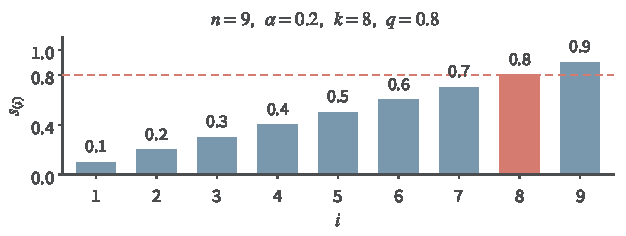
\includegraphics[width=106mm]{figures/02-foundations/03-trustworthiness/matplotlib/trust-conformal-residuals.pdf}};
 \draw[foundation flow] (63.5,52)--(63.5,44);
 \draw[foundation flow] (106.5,52)--(106.5,44);
 \draw[trust module,fill=white] (140,71) rectangle (167,79);
 \node at (153.5,75) {新输入$\bm x$};
 \draw[trust module] (138,53) rectangle (169,63);
 \node at (153.5,58) {$f(\bm x)$};
 \draw[foundation flow] (153.5,71)--(153.5,63);
 \draw[foundation flow,rounded corners=2mm] (63.5,70)--(63.5,81)--(132,81)--(132,58)--(138,58);
 \draw[trust module,fill=FigureYellowFill] (120,8) rectangle (169,39);
 \node at (144.5,34) {$C(\bm x)$};
 \draw[draw=FigureYellow,line width=1.2pt] (128,23)--(161,23);
 \draw[draw=FigureYellow,line width=1.2pt] (128,21)--(128,25) (161,21)--(161,25);
 \fill[FigureYellow] (144.5,23) circle (1.2);
 \node at (128,15) {$f(\bm x)-q$};
 \node at (144.5,19) {$f(\bm x)$};
 \node at (161,15) {$f(\bm x)+q$};
 \draw[foundation flow] (110,23)--(120,23);
 \draw[foundation flow] (153.5,53)--(153.5,39);
\end{tikzpicture}%

  \caption{拆分共形预测的构造。评分函数先由独立训练数据确定，再用校准分数选择阈值。图中采用教学残差$0.1,0.2,\ldots,0.9$，取$n=9$、$\alpha=0.2$，故$k=8$、$q=0.8$；绝对残差评分产生右侧回归区间。数值说明排序与集合构造，不是覆盖率的实验测量。}
  \label{fig:trust-conformal-construction}
\end{figure*}

\paragraph{自适应范围与条件覆盖边界}

边际覆盖建立后，还有两个需要分别回答的问题：集合能否随输入难度调整，以及能否把覆盖承诺落实到局部人群。前者关乎信息量，后者关乎保证范围；区间宽度自适应并不能自动解决后者。

固定宽度区间容易在低噪声区域过宽、在高噪声区域过窄。Romano、Patterson和Candès提出\term{共形分位数回归}（conformalized quantile regression, CQR），把前面学习到的上下分位点作为区间形状，再用共形分数修正覆盖\scite{romano2019cqr}。

具体地，先在训练集上拟合下、上分位点$\hat q_{\mathrm l}(\bm{x})$和$\hat q_{\mathrm u}(\bm{x})$，并保证两者顺序正确。校准分数取为
\begin{equation}
 s(\bm{x},y)
 =\max\{\hat q_{\mathrm l}(\bm{x})-y,\,
              y-\hat q_{\mathrm u}(\bm{x})\}.
 \label{eq:reliability-cqr-score}
\end{equation}
目标落在原区间外时，分数是越界距离；落在内部时，分数非正。按式~\eqref{eq:reliability-conformal-set}得到分位阈值$q$后，校准区间为
\[
 [\,\hat q_{\mathrm l}(\bm{x})-q,\,
       \hat q_{\mathrm u}(\bm{x})+q\,].
\]
正$q$扩张原区间，负$q$则允许收缩，必要时集合可以为空。有限样本边际覆盖来自相同的排序论证，不需要分位数模型拟合正确；区间是否短而有用，则依赖基础分位点能否反映局部噪声。

假设两个输入的原始区间分别为$[8,12]$和$[0,20]$，共形修正值为2，校准后区间就是$[6,14]$和$[-2,22]$。二者共享同一覆盖修正，却保留不同难度对应的宽度。这说明“有效性不依赖模型正确”与“效率依赖模型质量”能够同时成立。它仍不表示两个输入各自都获得规定的条件覆盖。

分类问题也需要让集合随难度变化。Romano、Sesia和Candès研究按类别概率的累计质量构造自适应预测集合：高概率类别集中时，只需少数类别；概率分散时，应保留更多可能性\scite{romano2020adaptivecoverage}。

例如，将类别按概率从大到小排序，候选类别的分数可以取截至该类别的累计概率，再使用独立样本校准阈值；原方法还通过随机化处理边界类别。若只按固定单类概率设阈值，不同输入上被排除的总概率质量可能差异很大。累计质量评分改善这一点，但基础概率错误时，仍只能依赖共形步骤提供边际有效性，不能把自适应集合误读成逐输入保证。

为何不能继续要求每个输入都准确覆盖？Barber等研究了无分布假设的条件预测推断限制：在足够一般的连续输入、实值输出问题中，要对所有分布提供非平凡的精确条件覆盖，存在根本障碍\scite{barber2020conditional}。

困难来自有限样本无法识别每个细小邻域中的结果分布。两个总体可以在所有已观察数据附近表现相同，却在尚未充分观察的输入区域有不同的尾部。若区间必须同时保护所有可能总体，就可能不得不变得极宽。增加神经网络规模无法自动解除这一信息限制；必须增加平滑性或分布假设，或放宽保证对象。

一种可行放宽是预先规定有限群体，在每个群体内单独校准；另一种是要求在一族受限切片上近似满足覆盖。群体越细，局部有效性越有针对性，但每组样本越少，集合也越保守。对预先规定的组，组内交换性支持相应组内覆盖；对看完错误再挑出的任意子组，不能直接沿用同一个论证。这一差别将在公平性章节再次出现：总体的好表现不能替代对特定受影响群体的证据。

\paragraph{变化环境中的长期覆盖}

部署后不断得到新标签时，固定阈值未必适合持续变化的数据。Gibbs和Candès提出\term{自适应共形推断}（adaptive conformal inference, ACI），用已经观察到的覆盖错误更新下一轮的名义错误水平，目标转向长期覆盖频率\scite{gibbs2021aci}。

令目标错误比例为$\alpha$，第$t$轮内部使用的名义水平为$a^{(t)}$，实际未覆盖指示为$e_t=\mathbb I\{y_t\notin C_t(\bm{x}_t)\}$。一个基本更新为
\begin{equation}
 a^{(t+1)}=a^{(t)}+\gamma(\alpha-e_t),
 \qquad \gamma>0.
 \label{eq:reliability-aci}
\end{equation}
发生未覆盖时，$a^{(t)}$减小，下一轮要求更高覆盖，集合趋于扩大；覆盖成功时则逐渐提高名义错误水平。将递推式相加可得
\[
 \frac1T\sum_{t=1}^{T}e_t-\alpha
 =\frac{a^{(1)}-a^{(T+1)}}{\gamma T}.
\]
只要内部状态始终有界，右侧就随$T$增大而趋于零。这是反馈控制的代数性质，并不要求每一轮数据独立同分布。

有界性不能被略去。原方法把分位数函数扩展到通常概率范围之外：名义错误水平小于0时允许输出全集，大于1时允许输出空集，以把更新推回范围。不能随意将$a^{(t)}$截断到$[0,1]$后，仍直接套用上面的无截断恒等式。全集和空集也说明了保证的代价：长期比例正确，未必意味着每轮集合都有用。

学习率$\gamma$决定反馈速度。较大值能更快响应变化，也带来更剧烈的集合波动；较小值更平稳，但可能在突变后恢复较慢。标签延迟、只有被接受样本才有反馈，或错误集中发生在某类输入时，还需要重新分析可观察性和目标。长期平均覆盖不能保护任意短时间窗口，更不能直接保证某一封高损失邮件处理正确。

\subsection{决策程序的风险保证}

上一小节保证真实结果进入集合，实际系统却还需要决定采取什么行动。覆盖错误只是任务损失的一种。共形风险控制把拆分共形的校准思想推广到参数化损失族，但具体保证还取决于损失有界性、风险随参数的单调结构、校准样本关系和所采用的选择规则\scite{angelopoulos2024crc}。本章不在这些条件尚未展开时把它当作已证明的风险证书；下面实际建立的是另一种结论：对验证前固定的有限候选程序，同时给出高概率期望风险上界。

\paragraph{固定候选程序的高概率风险界}

要理解高概率风险保证，可以从有限候选程序的选择开始。将预测器、接受阈值和拒答规则合起来视为一个程序；每个程序都在独立验证前固定，再用统一置信上界判断哪些程序可以投入使用。设$K$个程序在验证前固定，第$j$个程序的损失$L_j$取值于$[0,1]$，期望风险为$R_j=\mathbb E[L_j]$，验证样本独立同分布。记经验损失为$\hat R_j$，则Hoeffding不等式与联合界给出
\begin{equation}
 \mathbb P\left(
  \forall j,\ R_j\leq
  \hat R_j+\sqrt{\frac{\log(K/\delta)}{2n}}
 \right)\geq1-\delta.
 \label{eq:reliability-finite-program-bound}
\end{equation}
因为每个程序违反其上界的概率至多为$\delta/K$，全部违反事件的概率之和不超过$\delta$。
因此，可以在上界不超过目标风险的程序中，选择\emph{验证集经验处理比例}最高的一个，
而不破坏已经同时建立的风险界。这个选择并没有给总体处理比例提供置信保证；若服务能力
也是部署承诺，还须同时为$\mathbb E[A_j]$建立下置信界，并按风险上界与处理比例下界共同
筛选。若没有程序达标，应报告证据不足或改变处理策略，而不应只选经验风险最小者并宣称达标。

这一保证需要候选程序没有利用同一验证集任意生成。对零一预测损失，拒答若被计为零损失，上界控制的是全体请求中接受且出错的概率；这与式~\eqref{eq:reliability-selective-risk}中以接受请求为分母的条件风险不同。完整系统也可以把拒答成本纳入$L_j$，在归一化到$[0,1]$后比较风险与服务能力。

\paragraph{自动处理部分的条件风险界}

若使用要求明确针对自动处理部分，可以同时控制分子与分母。令第$j$个固定程序的接受指示为$A_j(\bm{x})\in\{0,1\}$，其预测损失为$\ell_j\in[0,1]$，记验证集上的联合损失均值为$\hat J_j=n^{-1}\sum_i A_j(\bm{x}_i)\ell_j(\bm{x}_i,y_i)$，接受比例为$\hat c_j=n^{-1}\sum_i A_j(\bm{x}_i)$。对$K$个分子的上界和$K$个分母的下界同时应用集中不等式，令$b_n=\sqrt{\log(2K/\delta)/(2n)}$，则以至少$1-\delta$的概率，对所有满足$\hat c_j>b_n$的候选程序都有
\begin{equation}
 R_{\mathrm{sel},j}
 =\frac{\mathbb E[A_j\ell_j]}{\mathbb E[A_j]}
 \leq\min\left\{1,\frac{\hat J_j+b_n}{\hat c_j-b_n}\right\}.
 \label{eq:reliability-conditional-risk-bound}
\end{equation}
这给出了按条件风险筛选程序的一种保守办法。接受比例很小时，分母下界接近零，保证会变弱；$\hat c_j\leq b_n$时，这一构造无法给出有用的条件风险上界。它不是模型一定不可靠的证明，而是当前样本和界不足以支持该承诺。扩大独立验证样本、改变接受规则或采用更适合该损失的置信界，才能进一步缩小证据缺口。

\paragraph{候选程序的构造与独立验证}

这一上界说明怎样筛选程序，却没有保证候选集合中一定存在足够好的程序。要扩大可行选择，还需在独立训练阶段构造更好的候选对象。候选程序既可以是固定预测器配上不同接受阈值，也可以通过训练联合学习预测与拒答。仅对现有分数设阈值，未必能得到适合筛选高风险输入的表示。Geifman和El-Yaniv提出的SelectiveNet把预测与选择联合训练，直接优化接受区域上的表现，而非仅在训练结束后按置信度截断\scite{geifman2019selectivenet}。

为了理解这类目标，令$g_i\in[0,1]$为样本的软接受权重，$\ell_i$为预测损失，目标处理比例为$c_0$，可以考察
\begin{equation}
 \frac{\sum_i g_i\ell_i}{\sum_i g_i}
 +\lambda\left(\max\left\{0,c_0-\frac1n\sum_i g_i\right\}\right)^2,
 \label{eq:reliability-selective-training}
\end{equation}
其中$\lambda>0$，并要求分母为正。第一项鼓励留下易于可靠处理的输入，第二项惩罚处理比例不足。为了避免网络在特征尚未学好时就只关注一个狭小子集，SelectiveNet还使用辅助预测头，在全部训练样本上学习同一预测任务，再将辅助损失与选择性损失加权结合。这是训练目标，而不是测试条件风险保证；模型仍需在独立数据上选择实际阈值并验证风险。

因此，训练、验证和选择各有职责：训练改善候选程序的风险与处理能力，独立验证构造上界，选择规则在同时有效的上界中确定可用程序。若看到验证结果后继续训练新候选，就已经改变了保证所依赖的数据关系，需要新的验证数据或另行处理这种适应性。

\subsection{两类保证的比较与适用边界}

预测范围保证把输出对象设为集合$C(\bm{x})$，控制真实结果未落入集合的事件。集合大小或区间长度决定这一保证是否仍有信息量，却不属于覆盖率本身。决策风险保证则把预测器、接受规则和后续行动合成一个程序，直接控制事先定义的损失。它可以把误判、拒答成本或其他行动后果纳入同一风险对象，却不要求程序一定输出预测集合。

保证对象并不决定概率量词和数据条件；同一种覆盖或风险对象，在不同数据制度下也可能对应不同结论。本节选取的拆分共形预测在校准样本与新样本可交换时提供边际覆盖，自适应共形推断在可观察反馈和有界内部状态下控制长期未覆盖频率，有限候选程序的高概率风险界则依赖独立同分布的验证样本，并对验证集的抽取给出置信要求。这些结论分别回答一次预测、长期序列和程序验证中的问题，不能只按数值大小比较强弱。

预测集合可以作为决策程序的输入，但覆盖保证不会自动变成行动风险保证。要从前者推出后者，还需说明程序怎样使用集合，以及覆盖失败、集合过大和拒答分别造成什么损失。反过来，一个通过独立验证的低风险程序也未必给出具有频率含义的概率或覆盖集合。实际选择保证时，应从使用承诺出发：需要容纳真实结果，就规定覆盖事件和范围效率；需要限制自动处理的后果，就规定行动损失和处理比例；两项都需要时，应分别建立并检验，不能用一个指标替代另一个。

\section{本章小结}
\label{sec:reliability-summary}

章首的0.9必须对应明确事件，并通过数据检验其频率含义。不确定性小、准确率高和校准良好是不同性质，可靠性检验还需兼顾信息量。

结果波动与知识不足是不确定性的两类来源。后验近似与深度集成估计模型间的预测分歧，条件分布与分位数学习刻画给定模型中的结果波动；两者结合后形成预测分布或范围。它们提供了待检验的主张，而不是可靠性已经成立的证据。

可靠性检验从三个角度核查这些主张：校准、评分与覆盖检查数值含义，风险—处理比例曲线检查识别高风险预测的能力，局部条件下的复测检查总体结论是否掩盖重要群体。数值准确、筛选有效、结论在相关局部条件下仍有证据，这三方面相互补充，任何一个总体指标都不能代替其余判断。

预测范围覆盖与决策程序风险是两类不同的保证对象，其适用范围取决于概率量词、抽样条件和损失定义。共形方法把模型质量与边际有效性分开，却不能无条件实现逐输入覆盖；在线反馈可以维护长期比例，却允许短期失效。选择性训练只能改善候选程序，风险承诺仍需独立验证。生成任务还要区分措辞变化、语义分歧与事实错误。下一章将承接其中最关键的条件变化：当输入和环境离开既有数据的范围，模型性能与这些可靠性承诺会怎样改变。

\paragraph{延伸阅读}

Guo等关于神经网络概率校准的研究适合继续比较分类准确率与概率质量；Angelopoulos与Bates的共形预测综述则从有限样本覆盖出发，说明基础预测器、校准数据和集合效率各自承担什么职责\scite{guo2017calibration,angelopoulos2022conformal}。

若关注生成任务，可结合语义熵与共形风险控制的工作阅读。前者区分措辞变化和语义分歧，后者要求把开放输出转成明确风险对象；两条路线都不能把低不确定性直接解释为事实正确\scite{kuhn2023semantic,loaizaganem2026confgen}。
